\section{eo\-Incrementor\-Param$<$ T $>$ Class Template Reference}
\label{classeo_incrementor_param}\index{eoIncrementorParam@{eoIncrementorParam}}
an {\bf eo\-Updater}{\rm (p.\,\pageref{classeo_updater})} that is an {\bf eo\-Value\-Param}{\rm (p.\,\pageref{classeo_value_param})} (and thus OWNS its counter) Mandatory for generation counter in make\_\-checkpoint  


{\tt \#include $<$eo\-Updater.h$>$}

Inheritance diagram for eo\-Incrementor\-Param$<$ T $>$::\begin{figure}[H]
\begin{center}
\leavevmode
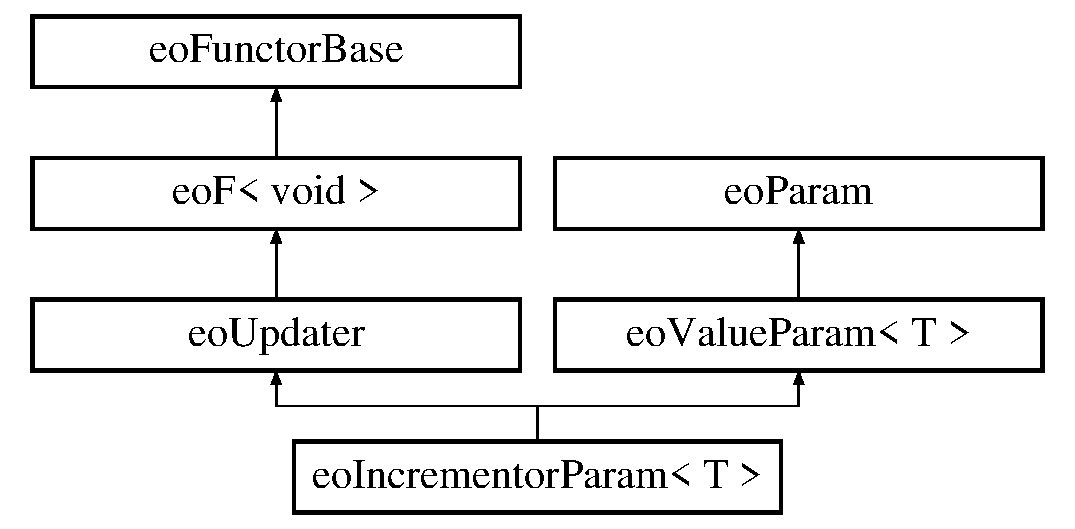
\includegraphics[height=4cm]{classeo_incrementor_param}
\end{center}
\end{figure}
\subsection*{Public Member Functions}
\begin{CompactItemize}
\item 
{\bf eo\-Incrementor\-Param} (std::string \_\-name, T \_\-stepsize=1)\label{classeo_incrementor_param_a0}

\begin{CompactList}\small\item\em Default Ctor : a name and optionally an increment. \item\end{CompactList}\item 
{\bf eo\-Incrementor\-Param} (std::string \_\-name, T \_\-count\-Value, T \_\-stepsize)\label{classeo_incrementor_param_a1}

\begin{CompactList}\small\item\em Ctor with a name and non-zero initial value and mandatory step\-Size to remove ambiguity. \item\end{CompactList}\item 
virtual void {\bf operator()} ()\label{classeo_incrementor_param_a2}

\begin{CompactList}\small\item\em Simply increments. \item\end{CompactList}\item 
virtual std::string {\bf class\-Name} (void) const \label{classeo_incrementor_param_a3}

\end{CompactItemize}
\subsection*{Private Attributes}
\begin{CompactItemize}
\item 
T {\bf stepsize}\label{classeo_incrementor_param_r0}

\end{CompactItemize}


\subsection{Detailed Description}
\subsubsection*{template$<$class T$>$ class eo\-Incrementor\-Param$<$ T $>$}

an {\bf eo\-Updater}{\rm (p.\,\pageref{classeo_updater})} that is an {\bf eo\-Value\-Param}{\rm (p.\,\pageref{classeo_value_param})} (and thus OWNS its counter) Mandatory for generation counter in make\_\-checkpoint 



Definition at line 71 of file eo\-Updater.h.

The documentation for this class was generated from the following file:\begin{CompactItemize}
\item 
eo\-Updater.h\end{CompactItemize}
